
\msection{Software diversification}
\label{sota:sw}


Software Diversification has been widely studied in the past decades. This section discusses its state-of-the-art.
% What is Software diversity
Software diversification consists in synthesizing, reusing, distributing, and executing different, functionally equivalent programs. 
According to the survey by Baudry \etal \cite{natural_diversity}, the motivation for software diversification can be separated in five categories: reusability \cite{pohl2005software}, software testing \cite{Chen2010AdaptiveRT}, performance \cite{10.1145/2025113.2025133}, fault tolerance \cite{1659219} and security \cite{cohen1993operating}. Our work contributes to the latter two categories. In this section we discuss related works by highlighting how they generate diversification and how they put it into practice. 

\todo{Work on differential testing}\url{https://arxiv.org/pdf/2309.12167.pdf}

%\lipsum[1]

%\lipsum[1]

\msubsection{Generation of Software Variants}


There are two primary sources of software diversification: Natural Diversity and Artificial Diversity\cite{natural_diversity}. This work contributes to the state of the art of Artificial Diversity, which consists of software synthesis. 
% Intro to Cohen and that functional/semantic equivalence is 
This thesis is founded on the work of Cohen in 1993 \cite{cohen1993operating} as follows.



% Mutation strategy
Cohen \etal \cite{cohen1993operating} proposed to generate artificial software diversification through mutation strategies.
A mutation strategy is a set of rules to define how a specific component of software development should be changed to provide a different yet functionally equivalent program. Cohen and colleagues proposed 10 concrete transformation strategies that can be applied at fine-grained levels. 
All described strategies can be mixed together. They can be applied in any sequence and recursively, providing a richer diversity environment. We summarize them, complemented with the work of Baudry \etal \cite{natural_diversity} and the work of Jackson \etal \cite{jackson}, in 5 strategies.

% A mutation can be applied at different layers of software lifecycle, from compilation to execution and from source code to executable binary.


%Natural diversity can be controlled or an unpredicted consequence of developing processes. Controlled natural diversity is usually called Design Diversity or N-Version Diversity. It is addressed using engineering decisions \cite{1659219}. 
%In practice, Natural Diversity consists of providing N development teams with the exact requirements. The teams develop N independent versions using different approaches. On the other hand, Natural Diversity can emerge from spontaneous software development processes. To illustrate the Natural Diversity phenomenon, CodeForces\footnote{\url{https://codeforces.com/contest/1667/status/page/2?order=BY_PROGRAM_LENGTH_ASC}} shows more than 350 different and successful solutions in C++ for a single requirements based problem in a single programming contest. 
%The software market is an expected source of natural diversity. Sengupta \etal \cite{10.5555/3091125.3091155} used this fact to reach the security goal (\autoref{goal:security}).



% Jump to the need of artificial
%Notice that Natural Diversity can rely on itself to escalate, and it is coped by the preexistence of software. This might be a limitation. For example, in the context o this work, the natural diversity for \wasm\ programs is nearly inexistence \cite{Hilbig2021AnES}. When natural diversity is not enough, it is innate to think that the source for diversification needs to be artificial. 

% Classification by Cohen



\begin{strategy}{Equivalent instructions replacement}
    \label{strategy:S1}
    \normalfont 
    Semantically equivalent code can replace pieces of programs. This strategy replaces the original code with equivalent arithmetic expressions or injects instructions that do not affect the computation result. There are two main approaches for generating equivalent code: rewriting rules and exhaustive searching. The replacement strategies are written by hand as rewriting rules for the first one. A rewriting rule is a tuple composed of a piece of code and a semantic equivalent replacement. For example, Cleemput \etal \cite{Cleemput2012} and Homescu \etal~\cite{homescu2013profile} insert NOP instructions to generate statically different variants. In their works, the rewriting rule is defined as \texttt{instr => (nop instr)}, meaning that \texttt{nop} operation followed by the instruction is a valid replacement .
    On the other hand, exhaustive searching samples all possible programs for a specific language. In this topic, Jacob \etal \cite{jacob2008superdiversifier} proposed the technique called superdiversification for x86 binaries. The superdiversification strategy proposed by Jacob and colleagues performs an exhaustive search of all programs that can be constructed from a specific language grammar. If one of the generated programs is equivalent to the original program, then it is reported as a variant. Similarly, Tsoupidi \etal \cite{Tsoupidi2020ConstraintBasedSD} introduced Diversity by Construction, a constraint-based compiler to generate software diversity for MIPS32 architecture.  
     %Their technique relies in using a constraint solver to generate program variants that by construction are semantically equivalent.
    %Compared to other techniques, the works of Jacob \etal and Tsoupidi \etal do not need the writing of replacement strategies by hand, but they are limited by the reach of theorem solvers and the generation of variants can only be static. 
    %An enumerative synthesis is a brute-force approach to generate program variants. With a maximum number of instructions, it constructs and checks all possible programs up to that limit. For a simplified instance, with a maximum code size of 2 instructions in a programming language with $L$ possible constructions, an enumerative synthesizer builds and checks all $L\times L$ combinations of programs. 
    %
\end{strategy}


\begin{strategy}{Instruction reordering}
    \label{strategy:S2}
    \normalfont
    This strategy reorders instructions or entire program blocks if they are independent.
    The location of variable declarations might change as well if compilers re-order them in the symbol tables. It prevents static examination and analysis of parameters and alters memory locations. In this field, Bhatkar \etal \cite{bhatkar03, bhatkar2005efficient} proposed the random permutation of the order of variables and routines for ELF binaries.
\end{strategy}

\begin{strategy}{Adding, changing, removing jumps and calls}
    \label{strategy:S3}
    \normalfont
    This strategy creates program variants by adding, changing, or removing jumps and calls in the original program. Cohen \cite{cohen1993operating} mainly illustrated the case by inserting bogus jumps in programs. Pettis and Hansen \cite{pettisochhansen} proposed to split basic blocks and functions for the PA-RISC architecture, inserting jumps between splits.
    Similarly, Crane \etal~\cite{crane2015thwarting} de-inline basic blocks of code as an LLVM pass. In their approach, each de-inlined code is transformed into semantically equivalent functions that are randomly selected at runtime to replace the original code calculation. On the same topic, Bhatkar \etal \cite{bhatkar2005efficient} extended their previous approach \cite{bhatkar03}, replacing function calls by indirect pointer calls in C source code, allowing post binary reordering of function calls. Recently, Romano \etal \cite{wobfuscator} proposed an obfuscation technique for JavaScript in which part of the code is replaced by calls to complementary Wasm function.
\end{strategy}


\begin{strategy}{Program memory and stack randomization}
    \label{strategy:S4}
    \normalfont
    This strategy changes the layout of programs in the host memory. Also, it can randomize how a program variant operates its memory. The work of Bhatkar \etal \cite{bhatkar03, bhatkar2005efficient} propose to randomize the base addresses of applications and the library memory regions in ELF binaries. Tadesse Aga and Autin \cite{aga2019smokestack}, and Lee \etal \cite{lee2021savior} propose a technique to randomize the local stack organization for function calls using a custom LLVM compiler.
    Younan \etal \cite{Younan2006} propose to separate a conventional stack into multiple stacks where each stack contains a particular class of
    data. 
    On the same topic, Xu \etal \cite{xu2020merr} transforms programs to reduce memory exposure time, improving the time needed for frequent memory address randomization. 
    %This makes it very hard for an attacker to ignore the key to inject executable code. This breaks the predictability of program execution and mitigates certain exploits. 
\end{strategy}


\begin{strategy}{ISA randomization and simulation}
    \label{strategy:S5}
    \normalfont
    This strategy uses a key to cypher the original program binary into another encoded binary. 
    Once encoded, the program can be decoded only once at the target client, or it can be interpreted in the encoded form using a custom virtual machine implementation. This technique is strong against attacks involving code inspection. 
    Kc \etal \cite{Kc03}, and Barrantes \etal \cite{barrantes2003randomized} proposed seminal works on instruction-set randomization 
    to create a unique mapping between artificial CPU instructions and real ones.
    On the same topic, Chew and Song \cite{Chew02mitigatingbuffer} target operating system randomization. They randomize the interface between the operating system and the user applications.
    Courouss{\'e} \etal~\cite{courousse2016runtime} implement an assembly-like DSL to generate equivalent code at runtime in order to increase protection against side-channel attacks. Their technique generates a different program during execution using an interpreter for their DSL.
    Code obfuscation \cite{wobfuscator} can be seen as a simplification of \emph{ISA randomization}. The main difference between encoding and obfuscating code is that the former requires the final target to know the encoding key while the latter executes as is in any client. Yet, both strategies are meant to tackle program analysis from potential attackers. 

    %It is an interpretation mechanism similar to encoding (\autoref{strategy:S9}), but the execution of programs is delegated to a custom interpreter instead of using preexisting execution hosts. The program is decoded at runtime every time it is invoked. 
    
\end{strategy}


\begin{comment}

\begin{strategy}{Intermixing}
    \label{strategy:S10}
    \normalfont
    With the existence of more than one program variant, the execution of program variants can be mixed. The decision of which variant executes is decided at runtime. This strategy is the core for randomization, multivariant execution and the execution by consensus defined in \autoref{goal:reliability}. This strategy is 
    complex to implement because the integrity of the memory and stack needs to be stable between programs.
\end{strategy}
\end{comment}
 



Equivalence checking between program variants is an essential component for any program transformation task, from checking compiler optimizations \cite{LeCompilers} to the artificial synthesis of programs discussed in this chapter. 
Equivalence checking proves that two pieces of code or programs are semantically equivalent \cite{churchill2019}. % Why is important
Cohen \cite{cohen1993operating} simplifies this checking by enunciating the following property: two programs are equivalent if given identical input, they produce the identical output. We use this same enunciation as the definition of \emph{functional equivalence} along with this dissertation. 
Equivalence checking in Software Diversification aims to preserve the original functionality for programs while changing observable behaviors. For example, two programs can be statically different or have different execution times and provide the same computation. 



% Humans, different DNA but similar as humans?
% The same feeling, the same performance, but some engine room parts and their connections are to some extent different.



% The relaxation of the equivalence checking
%Notice that this property is relaxed. Two programs can be statically different but still provide the same semantic output. For example, the work of Sengupta \etal \cite{sengupta} uses the rotation of different database engines for reliability. In this case, all database engines provide the same input/output property for creating, updating, and adding new data. Their solution has input/output equivalent programs provided by statically different binaries with different observable behaviors during runtime. On the contrary, the best example of restricted equivalence checking is the one followed by most antivirus applications. In practice, most of them check for the presence of the same binary in an enormous database, \ie if two programs are exactly the same binary, they are also semantically equivalent.


% Using the test suite and equivalence by construction
The equivalence property is often guaranteed by construction. For example, in the case illustrated in \autoref{strategy:S1} for Cleemput \etal \cite{Cleemput2012} and Homescu \etal \cite{homescu2013profile}, their transformation strategies are designed to generate semantically equivalent program variants. However, this process is prone to developer errors, and further validation is needed. For example, the test suite of the original program can be used to check the variant. If the test suite passes for the program variant \cite{harrand2020java}, then this variant can be considered equivalent to the original. However, this technique is limited due to the need for a preexisting test suite. When the test suite does not exist, another technique is needed to check for equivalence.

% Automatic equivalence checking SMT
If there is no test suite or the technique does not inherently implement the equivalence property, the previously mentioned works use theorem solvers (SMT solvers) \cite{SMT_solver} to prove equivalence. For SMT solvers, the main idea is to turn the two code variants into mathematical formulas. The SMT solver checks for counter-examples. When the SMT solver finds a counter-example, there exists an input for which the two mathematical formulas return a different output. The main limitation of this technique is that all algorithms cannot be translated to a mathematical formula, for example, loops. Yet, this technique tends to be the most used for no-branching-programs checking like basic block and peephole replacements \cite{SuperoptimizationScaling}.

% Automatic equivalence checking Fuzzers
Another approach to check equivalence between two programs similar to using SMT solvers is by using fuzzers \cite{zalewski2017american}.
Fuzzers randomly generate inputs that provide different observable behavior. If two inputs provide a different output in the variant, the variant and the original program are not equivalent. The main limitation for fuzzers is that the process is remarkably time-expensive and requires the introduction of oracles by hand.


%\todo{Move this to Technical chapter}
% Why SMT solvers
%We have found that SMT solvers are the best option for checking most of the fine-grained transformations previously mentioned for two main reasons. First, the field of SMT is mature and provides battle-tested tooling \cite{SMT_solver, SMTGupta}. Second, the existing SMT tooling is configurable and flexible, making the checking of program variants feasible in terms of the SMT solver execution time. In \autoref{chapter:technical} we describe how we apply SMT solvers in our contributions for equivalence checking.
%\subsection*{Vertical Software Diversification}

%\todo{Architecture level, remark these works but not in our scope.}
%The mentioned techniques can be applied at any layer of the software lifecycle, at coarse-grained or fine-grained levels.
%At high-level, Harrand \etal  \cite{harrand2020java}, propose to merge several Java decompiler variants to provide an extended and improved meta-decompiler. On the same topic, Sengupta \etal \cite{10.5555/3091125.3091155} shift several database engines and backends for web applications. Their idea makes known CVEs to be available only in certain time window, making potential attackers to not always success. Moreover, Roi \etal \cite{10.1145/3318216.3363338} proposed to use several machine learning algorithms with the same task to tackle adversarial attackers, using a different algorithm every time the system is queried.
%These works used preexisting software diversity to provide improved systems, both for reliability and security.


%\todo{Remove}
%For fine-grained diversification, the before mentioned mutation strategies can be applied directly to the basecode at the instruction level, during the compilation of programs or directly to the generated binaries. As we previously mentioned Homescu \etal \cite{homescu2013profile}, Jackson \etal \cite{jackson, jackson2011compiler}, Jacob \etal \cite{jacob2008superdiversifier}, Crane \etal \cite{crane2015thwarting}, Aga \etal \cite{aga2019smokestack} and Tsoupidi \etal \cite{Tsoupidi2020ConstraintBasedSD} placed compilers in their diversification techniques. Similarly, Bathkar \etal \cite{bhatkar03,bhatkar2005efficient}, Chew and Song \cite{Chew02mitigatingbuffer}, El-Khalil and Keromytis \cite{ElKhalil2004}, and Cohen \cite{cohen1993operating} itself mostly proposed binary to binary transformations. 
%We have observed that fine-grained techniques are mainly motivated because they provide more robust diversification in terms of preservation. For example, to apply diversification techniques closer to the final execution avoid removing of code transformations by later optimization or compilation stages. Our contributions are fine-grained based. 

%Superdiversifier, all the others, and then finish with that we contribute to fine-grained.




\begin{definition}{Software variant}
    \todo{Define}
\end{definition}
%\lipsum[1]

%\lipsum[1]

\begin{definition}{Uncontrolled diversification}
    \label{uncontroll_def}
    TODO
\end{definition}

\begin{definition}{Controlled diversification}
    \label{controlled_def}
    TODO
\end{definition}




\msubsection{Variants deployment}



After program variants are generated, they can be used in two main scenarios: Randomization or Multivariant Execution (MVE) \cite{jackson}. In \autoref{diagrams:sota:randomization} and \autoref{diagrams:sota:mve} we illustrate both scenarios. 



\newcommand{\rulesep}{\unskip\ \vrule\ }
\begin{figure}[h]
    \centering
    \begin{subfigure}[t]{0.45\textwidth}
        \centering
        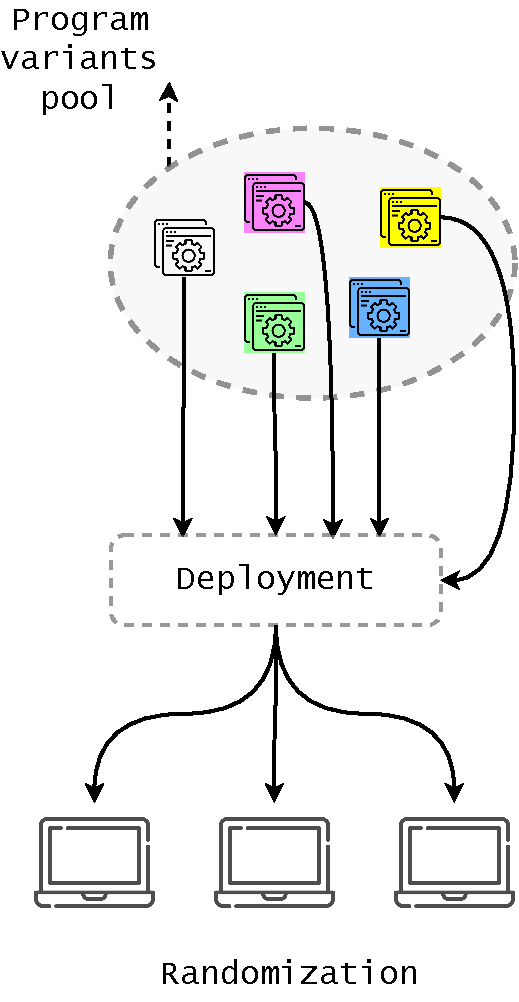
\includegraphics[height=3.1in]{diagrams/randomization.pdf}
        \vspace{0.5cm}
        \caption{Randomization scenario. Given a pool of program variants, one variant is deployed per host. Each deployment randomly selects which variant is assigned to each host. The same program variant is executed in the host at every program invocation between deployments. }        \label{diagrams:sota:randomization}

    \end{subfigure}
    \hspace{1.5mm}
    \rulesep
    \hspace{1.5mm}
    \begin{subfigure}[t]{0.45\textwidth}
        \centering
        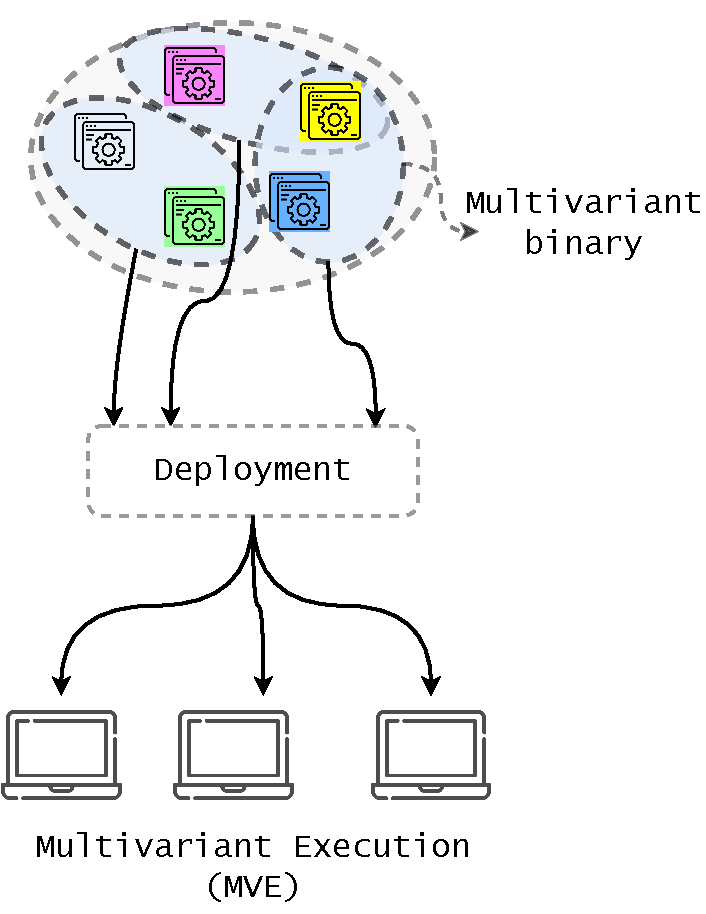
\includegraphics[height=2.8in]{diagrams/mve.pdf}
        \caption{Multivariant Execution scenario. Given a pool of program variants, a sample of the pool is packaged in a multivariant binary that is deployed. Each deployment randomly selects which multivariant binary is assigned to each host. Finally, a variant from the multivariant binary is randomly executed at runtime in the host.}        \label{diagrams:sota:mve}

    \end{subfigure}
    \caption{Software Diversification usages.}
\end{figure}

% \todo{Split in what and how?}

\begin{usage}{Randomization:}
    \label{usage:randomization}
    \normalfont
    % What
    In the context of our work \emph{Randomization} refers to the ability of a program to be served as different variants to different clients.
    % How
    In the scenario of \autoref{diagrams:sota:randomization}, a program is selected from the collection of variants (program's variant pool), and at each deployment, it is assigned to a random client. 
    % Why?
    Jackson \etal \cite{jackson} compare the variant's pool in Randomization with a herd immunity, since vulnerable binaries can affect only part of the client's community.

\end{usage}

% How to generate the variant's pool

El-Khalil and colleagues \cite{ElKhalil2004} propose to use a custom compiler to generate different binaries out of the compilation process. El-Khalil and colleagues modify a version of GCC 4.1 to separate a conventional stack into several component parts, called multistacks.
On the same topic, Aga and colleagues \cite{aga2019smokestack} propose to generate program variants by randomizing its data layout in memory. Their approach makes each variant to operate the same data in memory with different memory offsets.
The Polyverse company\footnote{\url{https://polyverse.com/}} materializes randomization at the commercial level in real life. They deliver a unique Linux distribution compilation for each of its clients by scrambling the Linux packages at the source code level.
    
% How
Virtual machines and operating systems can be also randomized. On this topic, Kc \etal \cite{Kc03}, create a unique mapping between artificial CPU instructions and real ones. Their approach makes possible the assignment of different variants to specific target clients. Similarly, Xu \etal \cite{xu2020merr} recompile the Linux Kernel to reduce the exposure time of persistent memory objects, increasing the frequency of address randomization.

%

    %This strategy prevents the usage of one variant to exploit another clients. When clients run two program variants, a potential attacker must create one attack for each variant. 
    %Therefore, the attacker must spend more time and effort to get the same return on reward for an attack. 
    %in their work they demonstrated that this usage can prevent against ROP and JIT-ROP attacks \citationneeded. Similarly, 
    % Amarilli \etal~\cite{amarilli2011can} drastically increase the number of execution traces required by a side-channel attack
    %To illustrate the impact of this usage, the Polyverse company \footnote{\url{https://polyverse.com/}} is able to provide unique Linux distributions to each one of their clients. 

\begin{usage}{Multivariant Execution (MVE):}
    \label{usage:mve}
    \normalfont
    % What
    Multiple program variants are composed in one single binary (multivariant binary) \cite{cox06}. Each multivariant binary is randomly deployed to a client. Once in the client, the multivariant binary executes its embedded program variants at runtime. \autoref{diagrams:sota:mve} illustrates this scenario. 
    
\end{usage}

% How, with two variants
The execution of the embedded variants can be either in parallel to check for inconsistencies or a single program to randomize execution paths \cite{bhatkar03}. 
Bruschi et al. \cite{bruschi2007diversified} extended the idea of executing two variants in parallel with not-overlapping and randomized memory layouts. Simultaneously, Salamat \etal \cite{salamat2007stopping} modified a standard library that generates 32-bit Intel variants where the stack grows in the opposite direction, checking for memory inconsistencies. 
Notably, Davi \etal proposed Isomeron \cite{davi2015isomeron}, an approach for execution-path randomization. Isomeron simultaneously loads the original program and a variant. While the program is running, Isomeron continuously flips a coin to decide which copy of the program should be executed next at the level of function calls. 
% More than two variants
The previously mentioned works showed the benefits of exploiting the limit case of executing only two variants in a multivariant environment.
Agosta \etal~\cite{agosta2015meet} and Crane \etal~\cite{crane2015thwarting} used more than two generated programs in the multivariant composition, randomizing software control flow at runtime. 

% More than two variants
 %has demonstrated to harden systems \cite{salamat2009orchestra, maurer2012tachyon}. Yet,  

%With Davi \etal approach, a potential attacker cannot predict whether the original or the variant of a program will execute.
% Their approach prevents against memory corruption. 
%Also, this system can be reached dynamically, like the work of Courouss{\'e} \etal, creating an MVE through code polymorphism \cite{10.1145/3281662}.  

%Besides, . 


%. Subsequent techniques focus on Multivariant. Execution for mitigating memory vulnerabilities \cite{lu2018stopping} and other specific security problems incl. return-oriented programming attacks \cite{volckaert2015cloning} and code injection \cite{SalamatJWWF11}. 

%

% Concluding the section
Both scenarios have demonstrated to harden security by tackling known vulnerabilities such as (JIT)ROP attacks \cite{jackson2011compiler} and power side-channels \cite{amarilli2011can}. Moreover, Artificial Software Diversification is a preemptive technique for yet unknown vulnerabilities \cite{jackson}. Our work contributes to both usage scenarios for \wasm.

%\begin{usage}{Moving Target Defense(MTD):}
%    \label{usage:mtd}
%    \normalfont
%\autoref{usage:randomization} and \autoref{usage:mve} can be categorized as Moving Target Defense strategies. Moving Target Defense for software was first proposed as a collection of techniques that aim to improve the security of a system by constantly moving its vulnerable components \cite{MTDNationalCyberLaep, okhravi2013survey}. Usually, MTD techniques revolve around changing system inputs and configurations to reduce attack surfaces. 
%This increases uncertainty for attackers and makes their attacks more difficult. Ultimately, potential attackers cannot hit what they cannot see. 
%MTD can be implemented in different ways, including via dynamic runtime platforms \cite{10.1145/3318216.3363338}. 
%In the case of \autoref{usage:n-version}, this usage lacks of the time dimension, \ie program variants are not changed from time to time. 

%\end{usage}

\todo{Multivariant}


\begin{definition}{Multivariant}
    \todo{Define}
\end{definition}

%\lipsum[1]

\todo{Automatic, SMT based}
\todo{Take a look to Jackson thesis, we have a similar problem he faced with the superoptimization of NaCL}
\todo{By design}
\todo{Introduce the notion of rewriting rule by Sasnaukas.}
\url{https://link.springer.com/chapter/10.1007/978-3-319-68063-7_13}


\msubsection{Defensive Diversification}

%\lipsum[1]

\msubsection{Offensive Diversification}


%\%todo{Esta muy regado ahora.}

%\todo{Stress input-output equivalence in the artificial diversification.}

%\todo{Mention concrete objective and achievement when citing.}

%\todo{emove some strategies, just cite some papers and thats it. Reduce to five transformations. Stick to U2 andd U3. Add techincal stack in the table.}

%\todo{Add level of transformation as a dimension. Hoigh level, fine-grained transofmrations, etc}

%\todo{Start with COhen, then go form high level to fine granied and from technologies to LLVM and Wasm.}


%\todo{Given a collection of pgorams, then enumerate the usages. Second approach, multiple encapsulation in one single program.}

%We finalize by comparing our contributions with the related work.

%\todo{Do not talk about complexity of replacements, stress them in the other chapters. Stress the comparison between techniques.}

%\todo{ Important things  }

%\todo{Rework hard sentences.}

%\todo{One section on semantically equivalence and checking...}

% \todo{Split sentences by ideas.}

%\subsection*{artificial software diversity.}

% Why we use their approach

\section{Open challenges}
\label{sota:openchallenges}

%We contribute to Software Diversification for \wasm\ using Artificial Diversification, for Randomization and Multivariant Execution usages (\autoref{usage:randomization}, \autoref{usage:mve}). 
In \autoref{table:sota:comparison} we list the related work on Artificial Software Diversification discussed along with this chapter. The first column in the table correspond to the author names and the references to their work, followed by one column for each strategy and usage (\autoref{strategy:S1},  \autoref{strategy:S2},  \autoref{strategy:S3},  \autoref{strategy:S4},  \autoref{strategy:S5}, \autoref{usage:randomization} and \autoref{usage:mve}). The last column of the table summarizes the technical contribution and the reach of the referred work. Each cell in the table contains a checkmark if the strategy or the usage of the work match the previously mentioned classifications. The rows are sorted by the year of the work in ascending order. 
In the following text, we enumerate the open challenges we have found in the literature research:
%The last two rows locate our contributions. 

%\input{sota/sota_table.tex}

% Move to introduction
%The primary motivation for our contributions is that we see in \wasm\ a monoculture problem. If one environment is vulnerable, all the others are vulnerable in the same manner as the same \wasm\ binary is replicated. 
%Besides, the \wasm\ environment lacks natural diversity \cite{natural_diversity}. Compared to the work of Harrand \etal \citationneeded, in WebAssembly, one could not use preexisting and different program versions to provide diversification. On the other hand, while the number of related work for software diversity is large, only one approach has been applied to the context of \wasm. 
% Move to the table
%To the best of our knowledge, the closest diversification work on the browsers involving \wasm\ is the work of Romano \etal \cite{wobfuscator}. They proposed to de-inline JavaScript subexpressions and replace them with function calls to \wasm\ counterparts. They empirically demonstrated that malware classifiers could be evaded with this diversification technique. 


\begin{enumerate}
    
    \item \emph{Software monoculture:}  
    The same Wasm code is executed in millions of clients devices through web browser.
    In addition, \wasm\ evolves to support edge-cloud computing platforms in backend scenarios, \ie replicating the same binary along with all computing nodes in a worldwide scale. Therefore, potential vulnerabilities are spread, highlighting a monoculture phenomenon \cite{Harrand1650630}. 

    \item \emph{Lack of Software Diversification for \wasm}:  Software Diversification has demonstrated to provide protection for known and yet-unknown vulnerabilities. However, only one software diversity approach has been applied to the context of \wasm\ \cite{wobfuscator}. 
    % Moreover, as we illustrate in \autoref{table:sota:comparison}, the existing works for software diversification do not contribute directly to \wasm.
    Moreover, \wasm\ is a novel technology and, the adoption of defenses is still under development \cite{Narayan2021Swivel, johnson2021} and has a low pace, making software diversification a possible preemptive technique.
    Besides, the preexisting works based on the LLVM pipeline cannot be extended to Wasm because they contribute to LLVM versions released before the inclusion of Wasm as an architecture. 
    % On the other hand, there is no mentioned work merging all mutation strategies in one solution.
    
    \item \emph{Lack of research on MVE for \wasm:} \wasm\ has a growing adoption for Edge platforms. However, MVE in a distributed setting like the Edge has been less researched. Only Voulimeneas \etal \cite{voulimeneas2021dmvx} recently proposed a multivariant execution system by parallelizing the execution of the variants in different machines for the sake of efficiency. 


\end{enumerate}






% Move this to the technical part
%CROW, extrapolates the idea of superdiversification \cite{jacob2008superdiversifier} for \wasm. CROW works directly with LLVM IR, enabling it to generalize to more languages and CPU architectures, something not possible with the x86-specific approach of previous works.
% CROW
%We contributes to state of the art in artificially creating randomization for \wasm\ (\autoref{usage:randomization}). 

%Due to the specificities of code execution in the browser (mentioned in \autoref{sota:wasm}), this can be considered as a randomization approach. For example, since \wasm\ is served at each page load, every time a user asks for a \wasm\ binary, she can be served a different variant provided by CROW. 
% Move to intro
%Besides, our contribution can be used in fuzzing campaigns \citationneeded to provide reliability. The diversification created by CROW can unleash hidden behaviors in compilers and interpreters. Thanks to CROW, a bug was discovered in the Lucet compiler \footnote{\url{https://www.fastly.com/blog/defense-in-depth-stopping-a-wasm-compiler-bug-before-it-became-a-problem}}.
%MEWE
%
% With MEWE \cite{MEWE}, our second contribution, we randomly select from several variants at runtime, creating a multivariant execution scheme(\autoref{usage:mve}) that randomizes the observable behaviors at each run of the multivariant binary. %We use the natural redundancy of edge-cloud computing architectures to deploy an internet-based MVE.

% Move to intro
% 

%CROW focuses on the static diversification of software. However, 



